\chapter{Planning}
This chapter includes the planning, the approach and the principle of a project that we have named ``\textbf{Fantasy}'', a web portal where teachers can perform a series of tasks (fantasies) with the objective that students can play and learn in a creative way.

The students will also have the possibility of creating the fantasies that the teacher sends them as work and then they will be evaluated by said professor.

\section{Development methodology}
The methodology used will be \ textbf {Scrum}: Agile development method characterized by having an incremental development and basing the quality of the result on knowledge rather than on the processes used.

\section{Project planning}
The project will last for three months and weekly meetings with the client will be held for a maximum of one hour.
\newpage
\begin{figure}[h]
	\centering
	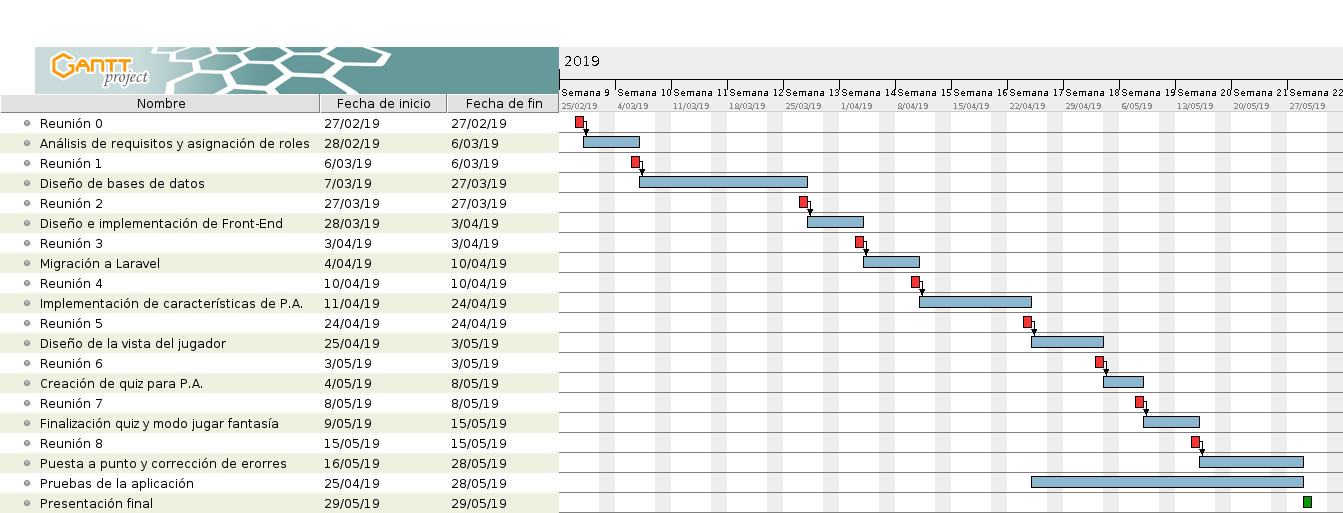
\includegraphics[scale=0.35]{Fantasy.png}
	\caption{Gantt diagram}
	\label{Gantt diagram}
\end{figure}

\section{Organization}
\subsection{Roles}
\begin{itemize}
	\item \textbf{Administrator:} Luis Gutiérrez Flores.
	\item \textbf{Analysts:} Jesús Rodríguez Heras and Nicolás Ruiz Requejo.
	\item \textbf{Designers:} Arantzazu Otal Alberro, Gabriel Fernando Sánchez Reina and Nicolás Ruiz Requejo.
	\item \textbf{Developers:} Luis Gutiérrez Flores, Alejandro Segovia Gallardo and Alejandro José Caraballo García.
	\item \textbf{Test Engineers:} Jesús Rodríguez Heras and Luis Gutiérrez Flores.
\end{itemize}

\subsection{Hardware and software resources}
As hardware resources we have the laptops of the 7 members of the group and the STIMEY server.

As software resources we have the framework Laravel, Atom, Visual Studio Code, TeXStudio, PhPMyAdmin, MySQL, GitHub.

\section{Costs}
\subsection{Human costs}
\begin{itemize}
	\item Hours in the learning of Laravel.
	\item PHP and MySQL training hours.
	\item GitHub training hours.
	\item Documentation hours.
\end{itemize}

\subsection{Material costs}
\begin{itemize}
	\item Our computers.
	\item Transportation to school.
	\item STIMEY server expenses.
\end{itemize}

\section{Risk management}
\begin{itemize}
	\item Do not meet deadlines for trying to cover too much and leaving incomplete functionalities.
\end{itemize}

\section{Team policy}
The team has decided to hold weekly meetings with the client, throughout the week, the team members will try to establish meetings between them with the necessary duration to continue advancing in the project (estimated time: two hours).

\section{Hits} %Seguir poniendo los demás sprints
\subsection{Sprint 0 ($27^{th}$ February to $6^{th}$ March)}
\begin{enumerate}
	\item Creation of work platforms and version control (GitHub).
	\item Creating the requirements sketch.
	\item Creation of use cases and their descriptions.
\end{enumerate}
\subsection{Sprint 1 ($6^{th}$ March to $27^{th}$ March)}
\begin{enumerate}
	\item Creation of platform mockups.
	\item Implementation of the database.
\end{enumerate}

\subsection{Sprint 2 ($27^{th}$ March to $3^{rd}$ April)}
\begin{enumerate}
	\item Implementation of front-end.
	\item Migrations of the database.
	\item Adaptation of the project to the Laravel framework.
	\item Creation of fantasies.
\end{enumerate}

\subsection{Sprint 3 ($3^{rd}$ April to $10^{th}$ April)}
\begin{enumerate}
	\item End of front-end.
	\item Final migrations of the database.
	\item Completion of fantasy creation.
\end{enumerate}

\subsection{Sprint 4 ($10^{th}$ April to $24^{th}$ April)}
\begin{enumerate}
	\item End of database migrations.
	\item Creation of active points with their basic characteristics.
\end{enumerate}

\subsection{Sprint 5 ($24^{th}$ April to $1^{st}$ May)}
\begin{enumerate}
	\item Creation of active points with all their characteristics.
	\item Start of the view to be able to play the fantasy.
\end{enumerate}


\section{Meetings}
\subsection{Meeting 0 ($27^{th}$ February)}
\begin{enumerate}
	\item Analysis of system requirements.
	\item Creation of use cases.
	\item Approach of the system database.
	\item Distribution of sprint tasks 0.
\end{enumerate}

\subsection{Meeting 1 ($6^{th}$ March)}
\begin{enumerate}
	\item End of sprint 0.
	\item Distribution of information to search.
	\item Start of sprint 1.
\end{enumerate}

\subsection{Meeting 2 ($27^{th}$ March)}
\begin{enumerate}
	\item End of sprint 1.
	\item Start of sprint 2.
\end{enumerate}

\subsection{Meeting 3 ($3^{rd}$ April)}
\begin{enumerate}
	\item End of sprint 2.
	\item Start of sprint 3.
\end{enumerate}

\subsection{Meeting 4 ($10^{th}$ April)}
\begin{enumerate}
	\item End of sprint 3.
	\item Start of sprint 4.
\end{enumerate}

\subsection{Meeting 5 ($24^{th}$ April)}
\begin{enumerate}
	\item End of sprint 4.
	\item Start of sprint 5.
\end{enumerate}
